%!TEX root = ../main.tex
% =============================================================
%  CAPÍTULO 4 — MARCO TECNOLÓGICO       (Entrega 4 · 10 % · 25/8)
% =============================================================

\chapter{Marco tecnológico}\label{cap:marco-tecnologico}

\begin{guia}[Guía de la cátedra: qué se evalúa en este capítulo]
Documenta el \emph{cómo}. No es un manual de uso: es la justificación
de cada elección tecnológica. Regla: nada ``porque sí''.
\begin{enumerate}
    \item \textbf{Arquitectura}: diagrama con componentes y conexiones,
          responsabilidad y tecnología de cada uno, flujo de datos y
          justificación del estilo arquitectónico con alternativas
          evaluadas \citep{sommerville2016}.
    \item \textbf{Prototipo o \gls{g:mvp}}: cuál es y por qué; alcance
          implementado vs.\ simulado; capturas o enlace; cómo se probó.
    \item \textbf{Stack}: por tecnología, nombre, versión, capa, por qué
          (madurez, comunidad, costo, conocimiento del equipo) y qué
          alternativas se descartaron.
    \item \textbf{Infraestructura y base de datos}: dónde se aloja cada
          componente, escalabilidad, costos (enlazados al
          capítulo~\ref{cap:economica}), motor y modelo de datos.
    \item \textbf{Diseño y \gls{ux}}: quién lo usa, mockups, decisiones de
          diseño y \textbf{cómo se validó con usuarios} (la cátedra lo marca
          como importante; cuestionario en el apéndice~\ref{apx:encuesta}).
    \item \textbf{Seguridad, calidad y despliegue}: autenticación, control
          de acceso, cifrado, plan de pruebas, repositorio, \gls{cicd} y
          monitoreo.
\end{enumerate}
\end{guia}

\section{Alcance del MVP y requisitos de diseño}

MotoSafe GBA cuenta con un MVP funcional en ejecución: backend, modelo
de gravedad, frontend y proceso de ingesta de prensa, con los tres
componentes corriendo en producción. El modelo de gravedad y el
extractor de prensa ya se midieron contra datos reales, con los
resultados y el detalle de cada medición en este mismo capítulo. El MVP
permite consultar el mapa con sus capas históricas y de contexto,
comparar rutas alternativas con su cobertura de datos declarada por
fuente, y reportar o consultar hechos recientes de prensa y reportes
comunitarios. El requisito transversal de diseño es que ninguna pantalla
presente ausencia de datos como bajo riesgo, ni una fuente incompleta
como si tuviera la misma certeza que una fuente histórica verificada.

\section{Arquitectura de contexto, contenedores y componentes}

El sistema se organiza en cuatro componentes independientes: un frontend
React/Vite con MapLibre que consume la API mediante peticiones HTTP; una
API FastAPI que carga en memoria el modelo Random Forest, sus columnas
de codificación y una tabla de contexto adicional por hotspot, y que
expone endpoints de consulta que leen los datos de hotspots y corredores
directamente de PostgreSQL en cada pedido; una base PostgreSQL con
PostGIS que persiste reportes comunitarios, noticias de prensa y
geometrías espaciales; y un proceso de scraping independiente que se
ejecuta periódicamente para descubrir, clasificar y geocodificar
noticias de fuentes periodísticas directas.

Esta separación de responsabilidades permite que un fallo del scraper no
derribe la API, y que un fallo transitorio de una capa secundaria
(inseguridad, corredores) no vacíe la capa principal de hotspots en la
interfaz. La composición productiva (docker-compose.production.yml)
aplica migraciones de base de datos antes de iniciar tanto la API como
el scraper, y no expone el puerto de la base de datos fuera de la red
privada del despliegue.

\begin{figure}[H]
    \centering
    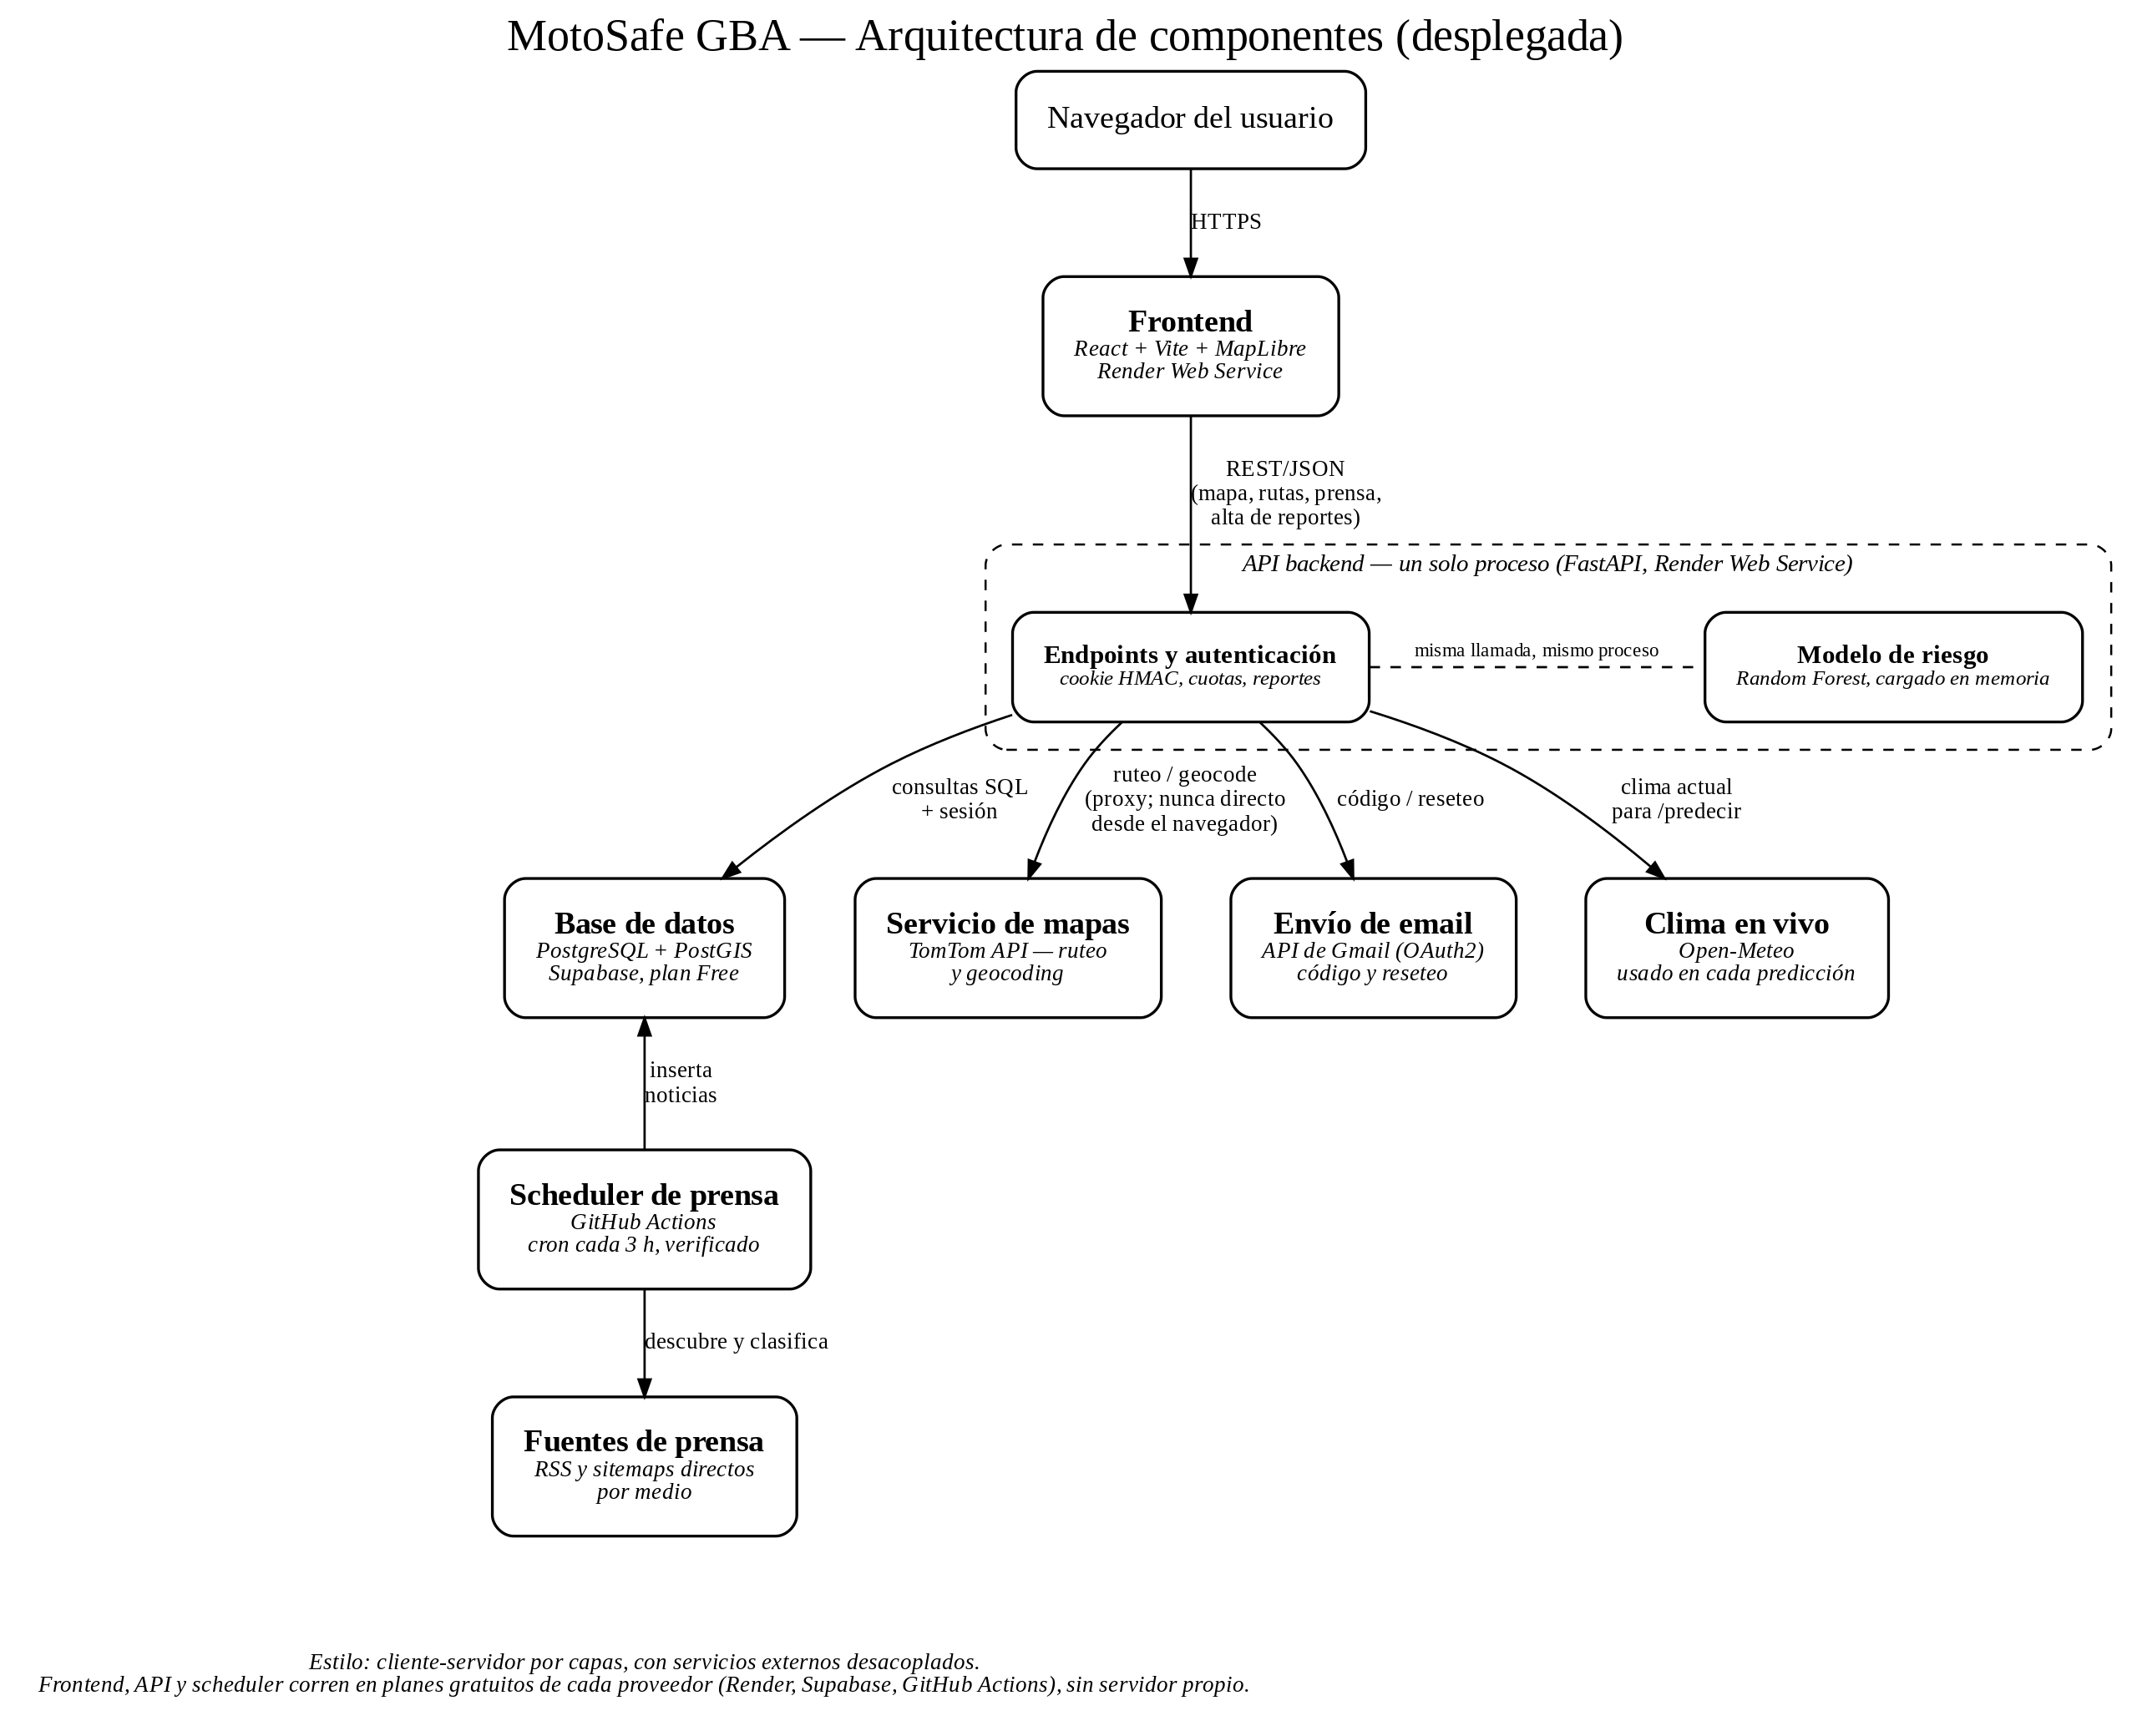
\includegraphics[width=0.9\textwidth,keepaspectratio]{figuras/image1.png}
    \caption{Arquitectura de componentes de MotoSafe GBA y flujo de datos entre ellos.}
    \label{fig:4-1}
\end{figure}

El estilo elegido es cliente-servidor por capas, con servicios externos
desacoplados detrás de la API; las alternativas descartadas para este y
otros componentes, con su justificación, se consolidan en 4.12.

\section{Criterios de selección tecnológica}

La selección tecnológica se evaluó según cinco criterios: capacidad de
representar información geográfica de forma nativa; compatibilidad con
un servicio web mantenible en el marco de un trabajo final de grado
desarrollado de forma individual; persistencia de geometrías y consultas
espaciales eficientes; trazabilidad de datos y cobertura de pruebas
automatizadas; y costo de una eventual operación sostenida más allá de
la entrega académica. Ningún criterio prueba por sí mismo la validez de
las estimaciones de riesgo que produce el sistema: aportan los medios
para presentar, consultar y auditar fuentes heterogéneas, no la
validación de esas fuentes.

El criterio de costo sostenible acota bastante el universo de opciones
frente a un proyecto que pudiera presupuestar una inversión inicial fija
y elegir, entre alternativas de mayor costo, la de mejor rendimiento
técnico. MotoSafe GBA no tiene ese margen: al ser un desarrollo
individual, en el marco de un trabajo final de grado, prioriza, en
igualdad de condiciones técnicas, la alternativa gratuita o de bajo
costo que se pueda mantener sin depender de un presupuesto externo,
incluso cuando esa alternativa ofrece menos capacidad que la opción de
mayor costo.

El criterio de mantenibilidad de un desarrollo individual también pesa
frente a la alternativa de resolver base de datos, autenticación y
funciones en la nube con una plataforma administrada única: ese tipo de
servicio reduce el trabajo de configuración cuando hay un equipo que se
reparte esa coordinación, pero MotoSafe GBA, como trabajo final de grado
desarrollado de forma individual, prioriza en cambio un stack que se
pueda operar de punta a punta sin depender de la disponibilidad de
terceros. Esta prioridad rige cómo se arma y se mantiene ese stack, no
dónde corre: la versión final del sistema se aloja íntegramente en la
nube, según se detalla en 3.8.

\section{Tecnologías seleccionadas: interfaz, mapa, API, datos, modelo y servicios externos}

Cada tecnología de esta sección se describe junto con la necesidad
funcional concreta que resuelve y, cuando corresponde, con la
alternativa considerada y descartada para el mismo problema.

\textbf{Interfaz: React con Vite}

Consultar y comparar información sobre un mapa, sin recargar la página
completa cada vez que cambia la capa o la ruta consultada, requiere una
interfaz que se ejecute como aplicación de una sola página (SPA): el
navegador carga la aplicación una vez y después actualiza solo las
partes de la pantalla que cambian. El proyecto utiliza React (una
biblioteca de JavaScript para construir interfaces a partir de
componentes reutilizables) con Vite (la herramienta que empaqueta y
sirve ese código durante el desarrollo y para producción) para eso. Una
aplicación móvil nativa fue descartada porque MotoSafe GBA no necesita
acceso a cámara, sensores de movimiento ni otras funciones exclusivas
del sistema operativo: la ubicación del usuario, que sí se usa para
centrar el mapa y calcular rutas, la provee directamente la API de
geolocalización del navegador, sin necesidad de una app nativa. Una
aplicación web evita, además, distribuir una app por tienda y llega al
usuario con un enlace.

\textbf{Mapa: MapLibre GL JS}

Mostrar el mapa y sus capas de forma interactiva, sin depender de un
proveedor cerrado de cartografía, requiere un motor de renderizado
propio, en línea con el criterio de trazabilidad discutido en 3.6;
MapLibre GL JS cumple ese rol: es una biblioteca de código abierto que
dibuja mapas vectoriales acelerados por GPU directamente en el
navegador. Nació como una continuación de Mapbox GL JS, el proyecto del
que se separó cuando este dejó de distribuirse bajo una licencia
abierta, y mantiene esa condición open source. Existen alternativas con
mejor rendimiento para volúmenes muy grandes de puntos por capa (decenas
o cientos de miles), pero MotoSafe GBA no maneja ese volumen de datos,
así que MapLibre GL JS es suficiente y evita la complejidad adicional de
una biblioteca pensada para escalas mayores a las que este proyecto
necesita.

\textbf{API y datos: FastAPI y PostgreSQL con PostGIS}

Exponer los recursos del sistema (consultas de hotspots, rutas, prensa,
reportes) a través de una API requiere un framework backend liviano; el
backend utiliza FastAPI (un framework de Python orientado a construir
APIs con validación de datos automática y buen desempeño). Persistir
reportes, noticias y geometrías con capacidad de consulta espacial
nativa (distancia, contención) requiere una base de datos con extensión
geoespacial; PostgreSQL con PostGIS cubre esa necesidad y constituye, en
la práctica, el estándar de facto para aplicaciones geoespaciales, con
más de 400 funciones de análisis espacial disponibles. Una plataforma
administrada que resuelva base de datos y backend como un único servicio
reduciría el trabajo de configuración inicial, pero a costa de menos
control sobre la lógica de negocio del lado del servidor; MotoSafe GBA
prioriza ese control.

\textbf{Modelo de gravedad: Python, pandas y scikit-learn}

El procesamiento de los datos históricos y el entrenamiento y evaluación
del modelo de gravedad usan Python, pandas (la biblioteca estándar de
Python para manipular datos tabulares) y scikit-learn, siguiendo las
prácticas de evaluación de esa misma biblioteca (scikit-learn
developers, s.f.) para evitar fuga de preprocesamiento. Es un stack de
aprendizaje automático clásico, no de aprendizaje profundo: los datos de
entrada son tabulares (hora, comuna, tipo de vía, clima, variables
demográficas), no imágenes ni secuencias con estructura espaciotemporal
compleja, así que un modelo de árboles como Random Forest (justificado
en 3.3) alcanza buen desempeño sin necesitar infraestructura de GPU ni
el volumen de datos que una red neuronal profunda requiere para entrenar
bien.

\textbf{Mapas y ruteo externos: TomTom}

Mostrar un mapa interactivo con búsqueda de direcciones y cálculo de
rutas reales no es algo que un proyecto de este alcance pueda construir
desde cero: se necesita una API externa de mapas y ruteo, y para eso el
proyecto utiliza TomTom, elegido por su capa gratuita más amplia para un
proyecto sin presupuesto de infraestructura, el mismo criterio de costo
sostenible descrito en 3.6. Su disponibilidad, cuota y costo se
mantienen documentados por separado de los datos propios del sistema,
porque su degradación o interrupción no debe interpretarse como una
falla del modelo de riesgo.

\section{Modelo de datos y procedencia}

El diseño de datos separa explícitamente registros históricos de
siniestros, artefactos entrenados del modelo, capas derivadas (hotspots,
corredores, inseguridad), rutas consultadas, reportes colaborativos y
noticias de prensa. Cada noticia conserva su fuente, URL de origen,
categoría temática, un atributo persistente e independiente
relacionado\_moto (verdadero solo cuando el título o la descripción
mencionan explícitamente una motocicleta), fecha editorial cuando la
fuente la declara, fecha de ingesta al sistema, y una precisión
geográfica categorizada.

Esta separación evita que una noticia se interprete como un dato oficial
de siniestralidad, o que una fuente de inseguridad general complete
artificialmente la cobertura histórica de una ruta. El flujo histórico
procesa los datasets de siniestros y publica consultas de referencia; el
flujo de prensa descubre notas en medios directos, aplica clasificación
textual y geocodificación acotada al área de CABA/GBA, deduplica de
manera conservadora dentro de una misma corrida, e inserta cada fila de
forma aislada mediante un savepoint (un punto de control de la
transacción de base de datos), de modo que una URL inválida se descarta
sin revertir el resto de la corrida.

\begin{figure}[H]
    \centering
    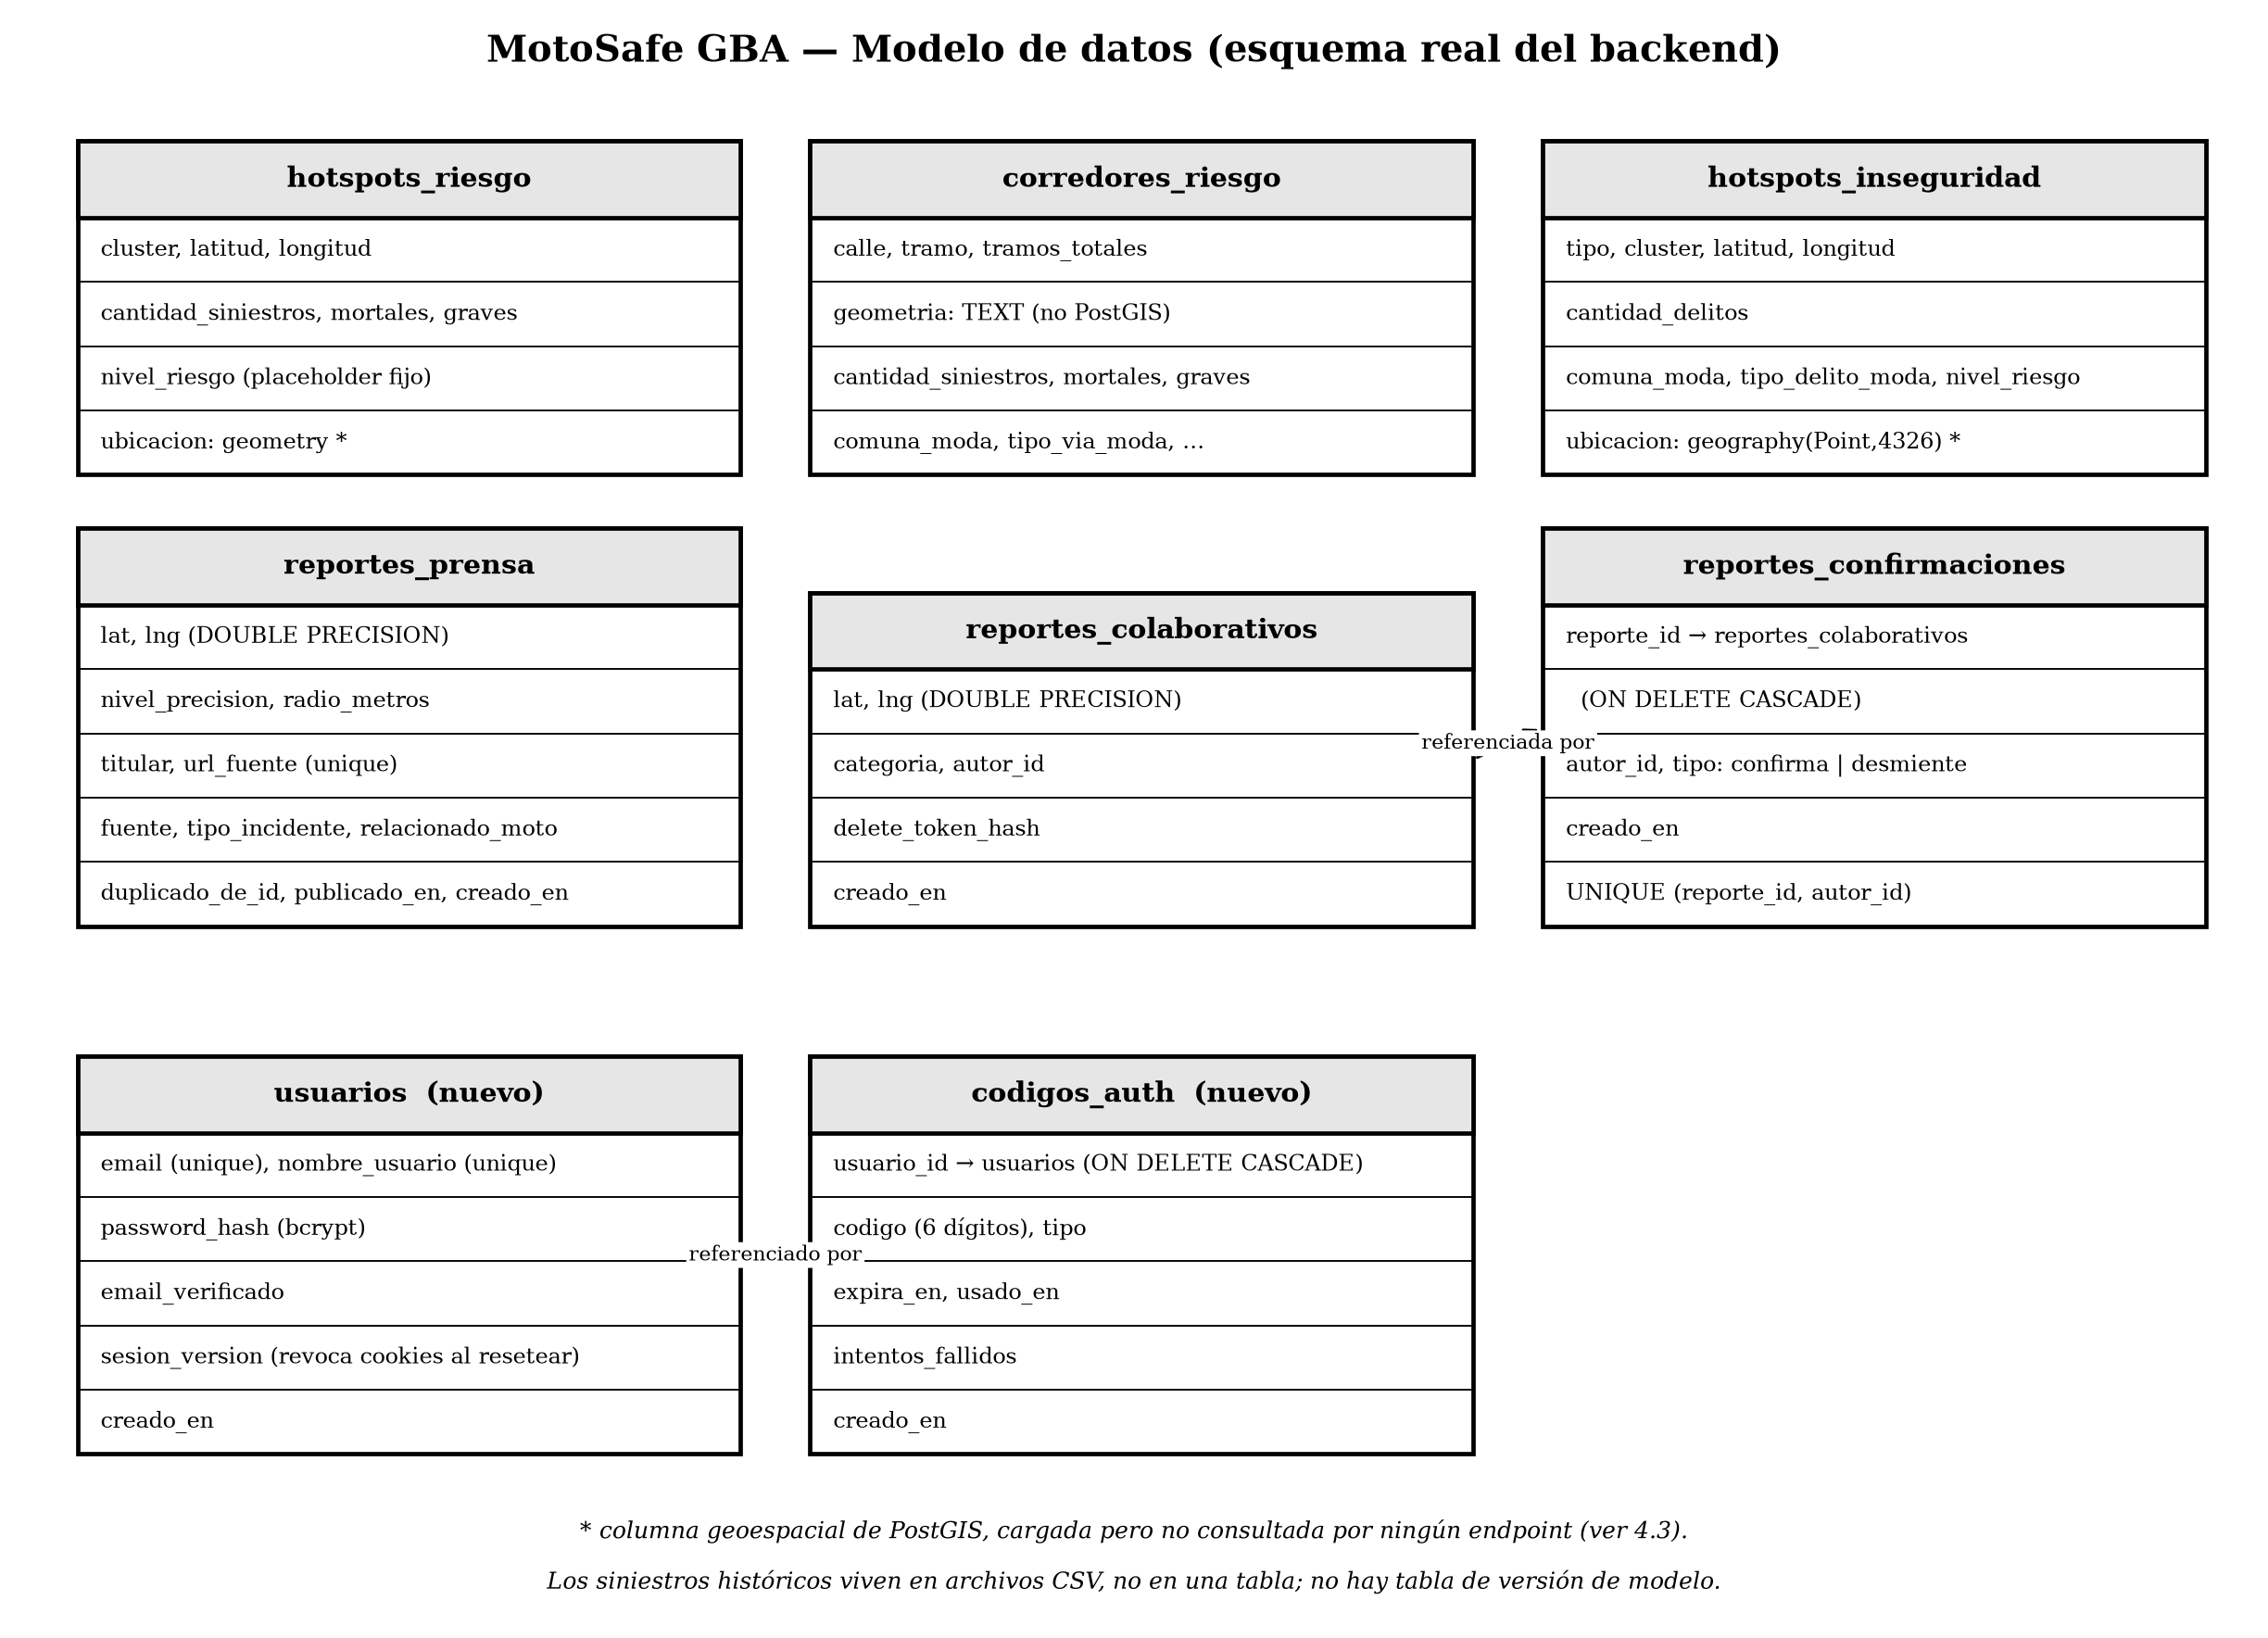
\includegraphics[width=0.9\textwidth,keepaspectratio]{figuras/image2.png}
    \caption{Modelo de datos del esquema real del backend, con los nombres de tabla y columnas tal como están hoy en PostgreSQL.}
    \label{fig:4-2}
\end{figure}

El motor de base de datos es PostgreSQL con la extensión PostGIS
habilitada. Las tablas centrales son hotspots\_riesgo y
corredores\_riesgo (capas de riesgo vial derivadas por agregación
espacial), hotspots\_inseguridad (capa de contexto de inseguridad
general), reportes\_prensa (noticias de prensa clasificadas) y
reportes\_colaborativos con reportes\_confirmaciones (reportes cargados
por usuarios y su validación por otros usuarios). Dos de esas tablas,
hotspots\_riesgo y hotspots\_inseguridad, ya guardan sus coordenadas
también como geometría nativa de PostGIS, pero el backend todavía no
aprovecha esa capacidad espacial: lee latitud y longitud como columnas
numéricas simples, y cuando necesita calcular proximidad (por ejemplo,
para ajustar el riesgo según reportes recientes cercanos a un punto) lo
hace con una fórmula matemática estándar, Haversine, en código Python,
no con una consulta espacial de PostGIS. Los siniestros históricos de
motociclistas que entrenan el modelo no están en una tabla de la base de
datos: se procesan aparte, como archivos CSV, en un pipeline que corre
fuera de línea (detalle en 4.4). El modelo entrenado tampoco tiene una
tabla propia de versiones: se guarda directamente como un archivo
serializado (pickle).

\section{Procesamiento de siniestros, modelo de gravedad y capas de riesgo}

El artefacto vigente es un RandomForestClassifier entrenado sobre 23.338
registros de siniestros con motocicleta cruzados con clima histórico. Su
configuración de hiperparámetros, ya fija, usa 300 árboles de decisión
combinados, con una profundidad máxima de 12 niveles por árbol y un
mínimo de 5 muestras por hoja (dos límites que evitan que el modelo
memorice casos particulares en vez de aprender un patrón general),
ponderación de clases balanced\_subsample (que compensa el desbalance
entre LEVE, GRAVE y MORTAL dándole más peso relativo a las clases
minoritarias en cada árbol) y semilla aleatoria fija en 42, para que el
resultado del entrenamiento sea reproducible. Usa 53 columnas de entrada
(se sacó la edad de la víctima y su indicador de edad desconocida,
porque esa variante generalizaba peor entre años que la que no las
incluye) que incluyen hora, temperatura, humedad, índice de inseguridad
general por comuna, día, comuna, tipo de vía, contraparte, sexo y
condición de lluvia, luego de codificación one-hot (una transformación
que convierte cada categoría, como el tipo de vía, en columnas separadas
de 0 y 1, porque el modelo no puede operar directamente con texto).

\begin{longtable}[]{@{}
  >{\raggedright\arraybackslash}p{(\columnwidth - 2\tabcolsep) * \real{0.5294}}
  >{\raggedright\arraybackslash}p{(\columnwidth - 2\tabcolsep) * \real{0.4706}}@{}}
\caption{Métricas del modelo de gravedad sobre la reconstrucción del split interno 80/20.}\label{tab:4-1}\\
\toprule\noalign{}
\begin{minipage}[b]{\linewidth}\raggedright
\textbf{Métrica (reconstrucción del split interno 80/20, n=4.668)}
\end{minipage} & \begin{minipage}[b]{\linewidth}\raggedright
\textbf{Resultado}
\end{minipage} \\
\midrule\noalign{}
\endfirsthead
\toprule\noalign{}
\begin{minipage}[b]{\linewidth}\raggedright
\textbf{Métrica (reconstrucción del split interno 80/20, n=4.668)}
\end{minipage} & \begin{minipage}[b]{\linewidth}\raggedright
\textbf{Resultado}
\end{minipage} \\
\midrule\noalign{}
\endhead
\bottomrule\noalign{}
\endlastfoot
Accuracy & 0,6262 \\
F1 macro & 0,368 \\
Recall / Precision GRAVE & 0,604 / 0,098 \\
Recall / Precision MORTAL & 0,464 / 0,105 \\
\end{longtable}

Estas cifras corresponden a una corrida archivada del artefacto vigente
sobre un split aleatorio interno (una partición al azar del mismo
conjunto de datos en una porción de entrenamiento y otra de evaluación,
sin separar por año), no a una evaluación temporal retrospectiva ni a
una prueba de generalización a GBA; esa es la distinción que importa en
este informe. Una reconstrucción posterior del mismo split y semilla
sobre el artefacto guardado hoy en el repositorio no reproduce estas
cifras de forma exacta (varían unas pocas centésimas en F1 macro y en
los recalls por clase); ambas corridas quedan documentadas con sus
artefactos en el repositorio, en vez de reemplazar un número por otro
sin trazabilidad.

Para saber si el modelo funciona igual de bien sobre datos que todavía
no vio, y no solo sobre los que ya usó para entrenarse, se lo evaluó
también separando los datos por año en lugar de al azar. Se ejecutó y
archivó ese protocolo de evaluación temporal retrospectiva, entrenando
sobre 2019-2022 (11.644 filas), reportando el desempeño sobre 2023
(3.915 filas) sin usar ese año para ajustar ningún hiperparámetro (la
configuración del modelo, 300 árboles, profundidad 12,
balanced\_subsample, se mantuvo fija e idéntica a la de producción en
las tres variantes evaluadas) y evaluando sobre 2024 como año
completamente posterior (3.331 filas), sin tocar el artefacto en
producción. La selección de la configuración final (qué variables
demográficas conservar) se apoyó en el desempeño observado sobre 2024 y
2025, así que esta evaluación se describe mejor como retrospectiva con
reuso para selección, no como una medición completamente ciega en ningún
paso del proceso. Este protocolo tampoco incluye el índice de
inseguridad por comuna entre las columnas de entrada, porque esa
variable no tiene todavía una versión fechada históricamente que pueda
reconstruirse año por año; el modelo que corre en producción sí lo usa.
La proporción de edad desconocida es del 45\% en entrenamiento y
selección, y del 12\% en el año de evaluación, una diferencia real de
completitud entre períodos que se declara como limitación de la
comparación.

\begin{longtable}[]{@{}
  >{\raggedright\arraybackslash}p{(\columnwidth - 6\tabcolsep) * \real{0.3696}}
  >{\raggedright\arraybackslash}p{(\columnwidth - 6\tabcolsep) * \real{0.2391}}
  >{\raggedright\arraybackslash}p{(\columnwidth - 6\tabcolsep) * \real{0.2391}}
  >{\raggedright\arraybackslash}p{(\columnwidth - 6\tabcolsep) * \real{0.1522}}@{}}
\caption{F1 macro y ECE por variante, evaluación temporal retrospectiva (selección 2023 y evaluación 2024).}\label{tab:4-2}\\
\toprule\noalign{}
\begin{minipage}[b]{\linewidth}\raggedright
\textbf{Variante}
\end{minipage} & \begin{minipage}[b]{\linewidth}\raggedright
\textbf{F1 macro (selección 2023)}
\end{minipage} & \begin{minipage}[b]{\linewidth}\raggedright
\textbf{F1 macro (evaluación 2024)}
\end{minipage} & \begin{minipage}[b]{\linewidth}\raggedright
\textbf{ECE}
\end{minipage} \\
\midrule\noalign{}
\endfirsthead
\toprule\noalign{}
\begin{minipage}[b]{\linewidth}\raggedright
\textbf{Variante}
\end{minipage} & \begin{minipage}[b]{\linewidth}\raggedright
\textbf{F1 macro (selección 2023)}
\end{minipage} & \begin{minipage}[b]{\linewidth}\raggedright
\textbf{F1 macro (evaluación 2024)}
\end{minipage} & \begin{minipage}[b]{\linewidth}\raggedright
\textbf{ECE}
\end{minipage} \\
\midrule\noalign{}
\endhead
\bottomrule\noalign{}
\endlastfoot
Con edad y sexo (base) & 0,348 & 0,262 & 0,318 \\
Sin edad & 0,317 & 0,286 & 0,304 \\
Sin edad ni sexo & 0,407 & 0,362 & 0,307 \\
\end{longtable}

Esta tabla evalúa por separado el efecto de sacar demografía, sin el
índice de inseguridad entre las columnas (ese protocolo todavía no lo
reconstruye año por año, como se explicó arriba). La variante con edad y
sexo cae a F1 macro 0,262 al evaluar sobre un año completo posterior al
de entrenamiento (intervalo bootstrap 95\%, el rango donde caería el
resultado si se repitiera la evaluación muchas veces sobre muestras del
mismo conjunto: [0,244; 0,281]), bastante por debajo de cualquier
reconstrucción de split aleatorio interno sobre el mismo período. La
variante que excluye solo la edad generaliza mejor entre años (F1 macro
0,286) que la que incluye demografía completa, y sacar también el sexo
mejora aún más (F1 macro 0,362), aunque a costa de buena parte del
recall de GRAVE (ver Tabla 4.3). La demografía disponible no aporta
señal estable entre años en este dataset: incluirla la degrada en vez de
mejorarla. El error de calibración (ECE) se mantiene en un rango similar
entre las tres variantes (0,30 a 0,32): las probabilidades predichas no
están bien calibradas en ninguna. Repitiendo esta misma comparación con
el índice de inseguridad incluido, para igualar el feature set real de
producción, la variante sin edad da F1 macro 0,3032 sobre 2024: es la
cifra que corresponde al modelo vigente, la que se usa en la Tabla 4.3.

Tabla: matriz de confusión del modelo sin edad (con sexo e índice de
inseguridad), la configuración vigente en producción, evaluación
temporal sobre 2024. Filas: clase real; columnas: clase predicha por el
modelo.

\begin{longtable}[]{@{}
  >{\raggedright\arraybackslash}p{(\columnwidth - 6\tabcolsep) * \real{0.2500}}
  >{\raggedright\arraybackslash}p{(\columnwidth - 6\tabcolsep) * \real{0.2500}}
  >{\raggedright\arraybackslash}p{(\columnwidth - 6\tabcolsep) * \real{0.2500}}
  >{\raggedright\arraybackslash}p{(\columnwidth - 6\tabcolsep) * \real{0.2500}}@{}}
\caption{Matriz de confusión del modelo sin edad, vigente en producción, evaluación temporal sobre 2024.}\label{tab:4-3}\\
\toprule\noalign{}
\begin{minipage}[b]{\linewidth}\raggedright
\textbf{Real / Predicho}
\end{minipage} & \begin{minipage}[b]{\linewidth}\raggedright
\textbf{GRAVE}
\end{minipage} & \begin{minipage}[b]{\linewidth}\raggedright
\textbf{LEVE}
\end{minipage} & \begin{minipage}[b]{\linewidth}\raggedright
\textbf{MORTAL}
\end{minipage} \\
\midrule\noalign{}
\endfirsthead
\toprule\noalign{}
\begin{minipage}[b]{\linewidth}\raggedright
\textbf{Real / Predicho}
\end{minipage} & \begin{minipage}[b]{\linewidth}\raggedright
\textbf{GRAVE}
\end{minipage} & \begin{minipage}[b]{\linewidth}\raggedright
\textbf{LEVE}
\end{minipage} & \begin{minipage}[b]{\linewidth}\raggedright
\textbf{MORTAL}
\end{minipage} \\
\midrule\noalign{}
\endhead
\bottomrule\noalign{}
\endlastfoot
GRAVE (n=210) & 126 & 54 & 30 \\
LEVE (n=3.078) & 1.360 & 1.464 & 254 \\
MORTAL (n=43) & 15 & 6 & 22 \\
\end{longtable}

La matriz muestra el patrón que explica la brecha entre precisión y
recall reportada arriba: el modelo sobre-predice GRAVE y MORTAL (recall
alto, 0,60 y 0,51) a costa de una precisión muy baja en esas dos clases
(0,08 y 0,07): de los 1.501 casos que el modelo marca como GRAVE, solo
126 lo son de verdad; de los 306 que marca como MORTAL, solo 22. Para un
sistema de alertas esto importa directamente: usar la predicción del
modelo como criterio único de aviso generaría muchos falsos positivos de
gravedad y mortalidad. La decisión de qué umbral de probabilidad dispara
una alerta, y qué costo relativo se le asigna a un falso positivo frente
a un falso negativo en cada clase, se tomó con evidencia cuantitativa:
se midió cómo cambian el recall y la precisión de MORTAL y de GRAVE a lo
largo de todo el rango posible de cortes de percentil. Esa medición
mostró que el recall de GRAVE cae de forma gradual sea cual sea el corte
elegido, mientras que el de MORTAL se mantiene alto hasta un punto
bastante más exigente y recién ahí empieza a bajar. Por eso el corte
vigente (percentil 75 para ``alto'', percentil 95 para ``crítico'') se
fijó priorizando no perder recall de MORTAL, aun a costa del recall de
GRAVE, que de todos modos iba a bajar con cualquier corte que se
eligiera.

Sobre este universo se derivan las capas de riesgo espacial: 740
hotspots viales (con el frontend reconsultando la capa cada cinco
minutos; los hotspots en sí se recalculan fuera de línea, no en cada
consulta), 243 corredores calculados fuera de línea, y una capa de
inseguridad general (633 hotspots, 502 con vinculación a motocicleta)
obtenida por clustering HDBSCAN sobre delitos de la Ciudad. El ajuste
por lluvia, que antes se aplicaba dos veces (en el backend y en el
frontend), se corrigió para aplicarse una sola vez.

Antes de promover un cambio en estos artefactos a producción, un script
de monitoreo (notebooks/monitor\_calidad\_datos.py) compara la versión
candidata contra la vigente y reporta, sin decidir ni bloquear nada por
su cuenta, tres tipos de cambio: de esquema (columnas nuevas,
desaparecidas o de tipo distinto), saltos relevantes en la proporción de
datos faltantes por columna, y saltos en la limpieza geográfica
(coordenadas inválidas, fuera del área de cobertura o duplicadas). Se
usó, por ejemplo, para confirmar que extender a los datos de delitos el
mismo criterio de limpieza geográfica que ya tenían los de siniestros no
introdujera ningún cambio de esquema inesperado antes de promover una
nueva versión de la capa de inseguridad (633→619 hotspots generales, 502
con vinculación a motocicleta sin cambios), que al cierre de esta
entrega quedó medida y verificada pero todavía sin aplicarse contra la
base real.

\section{Diseño de rutas, cobertura y comunicación de límites}

El comparador de rutas muestrea hasta 120 vértices de cada trazado
alternativo e informa, por separado, la proporción de esos vértices (no
de kilómetros recorridos) cercana a registros de siniestros y a
registros de inseguridad. Una fuente sin datos en una zona se muestra
como "sin datos", una categoría distinta de "0\%": el primer caso no
permite concluir nada sobre esa zona, mientras que el segundo indica que
la fuente disponible efectivamente no tuvo registros próximos bajo el
radio configurado. La recomendación de "menor exposición" exige un
mínimo de 60\% de cobertura sobre el eje histórico de siniestros; la
inseguridad general no reemplaza esa cobertura porque tiene procedencia,
unidad y significado distintos.

\section{Ingesta de prensa directa y reportes colaborativos}

\begin{figure}[H]
    \centering
    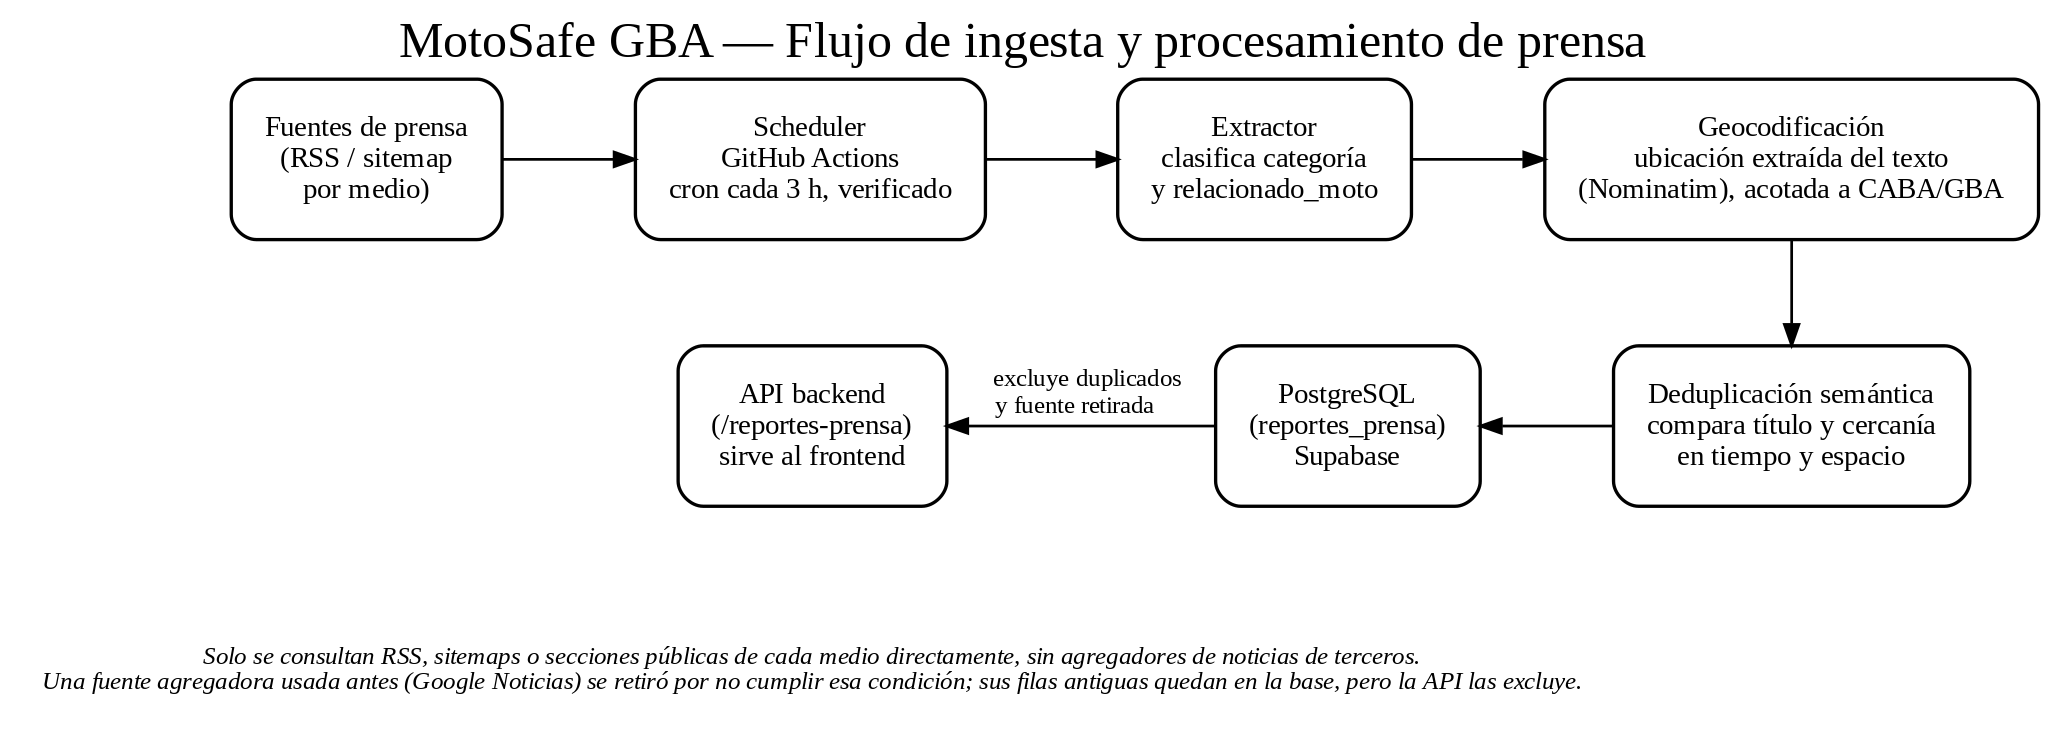
\includegraphics[width=0.9\textwidth,keepaspectratio]{figuras/image3.png}
    \caption{Flujo de ingesta y procesamiento de prensa, de la fuente a la API.}
    \label{fig:4-3}
\end{figure}

El proceso de ingesta consulta únicamente fuentes periodísticas directas
(RSS, sitemap o secciones públicas de cada medio), sin pasar por
agregadores de noticias de terceros: un agregador no garantiza que el
medio original autorice ese uso de su contenido, y una fuente directa
sí. Cada hallazgo se clasifica como robo, inseguridad o choque, con
relacionado\_moto como atributo independiente. Una fuente agregadora
usada antes (Google Noticias) se retiró por no cumplir esa condición;
sus filas antiguas quedan en la base, pero la API las excluye.

La calidad del extractor (precisión de clasificación, error geográfico)
se midió contra un conjunto etiquetado a mano (132 candidatas reales,
105 evaluables y 27 excluidas). La deduplicación semántica entre notas
equivalentes de medios distintos se midió contra 450 filas reales de la
base: a partir de un 70\% de palabras compartidas entre títulos de
fuentes distintas, el método identificó siempre el mismo hecho real, y
por debajo de un 45\% empezó a confundir hechos distintos del mismo
partido con el mismo tipo de incidente. Sobre esa medición se agregó una
marca automática que no borra ninguna fila: la nota duplicada se guarda
igual, pero queda excluida del mapa y del ajuste de riesgo por reportes
recientes. Falta confirmar ese comportamiento contra una corrida real de
producción.

\section{Diseño de interfaz, accesibilidad y experiencia de uso}

La interfaz sigue como referencia las Pautas de Accesibilidad para el
Contenido Web 2.2 del World Wide Web Consortium \citeyearpar{wcag2024} para foco visible, navegación por teclado y
tamaño de objetivos interactivos. El sistema implementa foco visible,
zoom nativo del navegador y respeto a la preferencia de movimiento
reducido del sistema operativo, y cuenta con una matriz de verificación
reproducible para teclado, zoom al 200\%, temas claro/oscuro, viewports
móviles y estados de red degradada. Esa matriz todavía no se ejecutó de
manera sistemática con dispositivos reales, así que su resultado queda
como protocolo pendiente de ejecución, no como validación cerrada.

\section{API, seguridad, privacidad y operación}

Esta sección resume los resguardos de seguridad, privacidad y operación
de la API, más allá de su función principal de servir datos. El endpoint
de salud (/health) informa estado del servicio, disponibilidad de la
base de datos, hora UTC y el estado de los umbrales de riesgo y la
versión de scikit-learn, sin exponer URLs, claves ni datos de usuarios.
El contenido externo (títulos y descripciones de prensa) se inserta como
texto en nodos DOM, sin interpretarse como marcado HTML, evitando la
ejecución de contenido inyectado. El borrado de un reporte comunitario
requiere un token privado de un solo uso entregado al autor del reporte
al momento de crearlo, en lugar de depender de un identificador que se
muestra públicamente; los reportes creados antes de este cambio no
tienen ese token y se mantienen así, sin una migración retroactiva. La
creación de reportes está sujeta a una cuota de 15 por dispositivo cada
24 horas (autor\_id, verificada antes del alta), pensada para cubrir el
abuso sostenido desde un mismo dispositivo que el límite por IP no
alcanza a cubrir, y el borrado de reportes quedó bajo el mismo límite de
frecuencia por IP que el resto de los endpoints de escritura. Un
endpoint /metrics, agregado la misma fecha, expone en memoria el conteo
de solicitudes, errores 4xx y 5xx, y la latencia promedio por ruta, sin
exponer configuración, tokens ni datos personales.

El pool de conexiones a la base de datos tiene un límite físico
configurado, tiempo de espera acotado y recuperación mediante rollback
ante una transacción abortada, verificado con una prueba unitaria; la
integración contra una instancia real de PostgreSQL bajo carga sigue
pendiente. Las entradas de la API (coordenadas, hora, edad) rechazan
valores fuera de rango, y una tabla de hotspots vacía no provoca un
error del modelo.

\subsection{Sistema de usuarios y autenticación real}

El sistema no depende de un usuario único fijo por variable de entorno:
tiene un esquema real de cuentas, con registro por email, nombre de
usuario y contraseña (hash bcrypt), verificación de la cuenta con un
código de 6 dígitos enviado por correo real (vence a los 15 minutos, con
un máximo de 5 intentos), inicio de sesión por email o por nombre de
usuario indistintamente, y reseteo de contraseña con el mismo mecanismo
de código. La sesión se mantiene con una cookie firmada (HMAC, sin
estado del lado del servidor) que incluye una versión de sesión
verificada contra la base en cada pedido protegido: cambiar la
contraseña incrementa esa versión y revoca de inmediato cualquier cookie
emitida antes del cambio, sin esperar a que venza su duración máxima de
12 horas. Un limitador de intentos por IP (5 cada 60 segundos, por
acción) cubre login, reenvío de código, pedido de reseteo y reseteo en
sí.

El envío de los códigos usa la API HTTP de Gmail (OAuth2 con un token de
larga duración) en vez de SMTP directo, porque Render bloquea el tráfico
saliente por los puertos SMTP en su plan gratuito; la API HTTP usa el
mismo puerto 443 que cualquier tráfico web y no está sujeta a esa
restricción. Todo el flujo se probó de punta a punta contra la
aplicación real en producción: registro, código real recibido y
confirmado leyendo la bandeja de entrada real, inicio de sesión, reseteo
de contraseña con otro código real, y una cookie emitida antes de un
reseteo efectivamente dejando de funcionar después de él. Captura real
de la pantalla de inicio de sesión en producción disponible en la
carpeta de evidencias del proyecto.

\section{Operación, contenedores y despliegue en producción}

Para reproducir el mismo entorno entre desarrollo y producción, con
servicios que puedan iniciarse, actualizarse y fallar de forma
independiente, el sistema se organiza en contenedores. Docker empaqueta
cada servicio con sus dependencias en una unidad aislada y reproducible,
y Docker Compose coordina el conjunto como un único sistema, con
servicios diferenciados para interfaz, API, base de datos y el proceso
periódico de ingesta de prensa.

Containerizar todo el sistema responde a operar sin equipo ni
presupuesto de infraestructura dedicado: un conjunto de servicios
administrados resolvería buena parte de esta operación, con el proveedor
encargándose de escalar y mantener la infraestructura a cambio de un
costo recurrente o de límites de uso gratuito más acotados. MotoSafe GBA
prioriza en cambio un stack que se pueda levantar de manera idéntica en
cualquier máquina y en cualquier proveedor de contenedores, sin atarse a
las particularidades de un servicio administrado específico.

El sistema está publicado y en funcionamiento en producción, con sus
tres componentes corriendo fuera de cualquier máquina local: la API y el
sitio web en Render (motosafe-api.onrender.com y
motosafe-web.onrender.com, como Web Services Docker del plan gratuito),
la base de datos en Supabase (PostgreSQL 17 con PostGIS, conectada por
el pooler de sesión para compatibilidad IPv4) y la tarea periódica del
scraper de prensa en GitHub Actions (cron cada tres horas), que
reemplaza al cron job de Render porque ese tipo de servicio es pago
incluso en el plan más chico de esa plataforma. La decisión de usar
Supabase en lugar de la base de datos propia de Render surgió de dos
hechos verificados en vivo, no de una preferencia a priori: la base
gratuita de Render vence a los 30 días (no sirve para una operación
sostenida) y Supabase ofrece un plan gratuito sin vencimiento con
PostGIS incluido. El manejo de secretos quedó fuera del repositorio
desde el principio (variables de entorno cargadas en el panel de cada
proveedor, nunca en Git).

\section{Prototipo funcional: evidencia visual}

Esta sección incorpora capturas de pantalla reales de la aplicación en
ejecución, tomadas sobre la aplicación real en producción
(motosafe-web.onrender.com), no sobre una instancia local. Las cuatro
figuras de esta sección quedan incluidas a continuación, con el detalle
de qué muestra cada una y qué evidencia aporta respecto de lo
documentado en 4.4 a 4.7.

Las cuatro figuras incorporadas, con la evidencia que cada una aporta,
son:

\begin{longtable}[]{@{}
  >{\raggedright\arraybackslash}p{(\columnwidth - 4\tabcolsep) * \real{0.1444}}
  >{\raggedright\arraybackslash}p{(\columnwidth - 4\tabcolsep) * \real{0.3889}}
  >{\raggedright\arraybackslash}p{(\columnwidth - 4\tabcolsep) * \real{0.4667}}@{}}
\caption{Figuras del prototipo funcional incorporadas y evidencia que aporta cada una.}\label{tab:4-4}\\
\toprule\noalign{}
\begin{minipage}[b]{\linewidth}\raggedright
\textbf{Figura}
\end{minipage} & \begin{minipage}[b]{\linewidth}\raggedright
\textbf{Qué debe mostrar}
\end{minipage} & \begin{minipage}[b]{\linewidth}\raggedright
\textbf{Evidencia que aporta}
\end{minipage} \\
\midrule\noalign{}
\endfirsthead
\toprule\noalign{}
\begin{minipage}[b]{\linewidth}\raggedright
\textbf{Figura}
\end{minipage} & \begin{minipage}[b]{\linewidth}\raggedright
\textbf{Qué debe mostrar}
\end{minipage} & \begin{minipage}[b]{\linewidth}\raggedright
\textbf{Evidencia que aporta}
\end{minipage} \\
\midrule\noalign{}
\endhead
\bottomrule\noalign{}
\endlastfoot
Figura 4.4 & Vista principal del mapa de MotoSafe GBA con al menos dos
capas de riesgo activas simultáneamente (por ejemplo, hotspots viales e
inseguridad general), sobre el área de CABA/GBA. & Evidencia visual de
que las capas de riesgo descritas en 4.4 y 4.5 se renderizan de forma
diferenciada y activable por separado, tal como se documenta en el
código. \\
Figura 4.5 & Panel de prensa con el filtro "Motos" aplicado, mostrando
noticias clasificadas por tipo de hecho (robo, inseguridad, choque) y el
atributo relacionado\_moto. & Evidencia de que el filtro Motos no oculta
el resto de la capa de prensa y de que la clasificación por tipo de
hecho descrita en 4.6 se refleja efectivamente en la interfaz. \\
Figura 4.6 & Comparador de hasta tres rutas alternativas, mostrando para
cada una el porcentaje de cobertura por fuente (siniestros históricos e
inseguridad) o la etiqueta "sin datos" cuando corresponda. & Evidencia
de que la distinción entre "sin datos" y "0\%" descrita en 4.5 se
comunica al usuario y de que el límite de interpretación de cobertura no
queda solo documentado sino visible en pantalla. \\
Figura 4.7 & Vista en un viewport móvil o un estado de red degradada
(por ejemplo, una capa secundaria sin poder actualizarse, con el aviso
correspondiente y los datos en caché conservados). & Evidencia del
comportamiento descrito en 4.7 y en CONTINUIDAD.md ante una fuente que
no puede actualizarse, y de la responsividad de la interfaz en pantallas
pequeñas. \\
\end{longtable}

Cada figura está numerada en secuencia (Figura 4.4 a 4.7), con título
descriptivo, correspondiente a la aplicación real en producción desde el
despliegue confirmado en 3.8 y 4.10.

\begin{figure}[H]
    \centering
    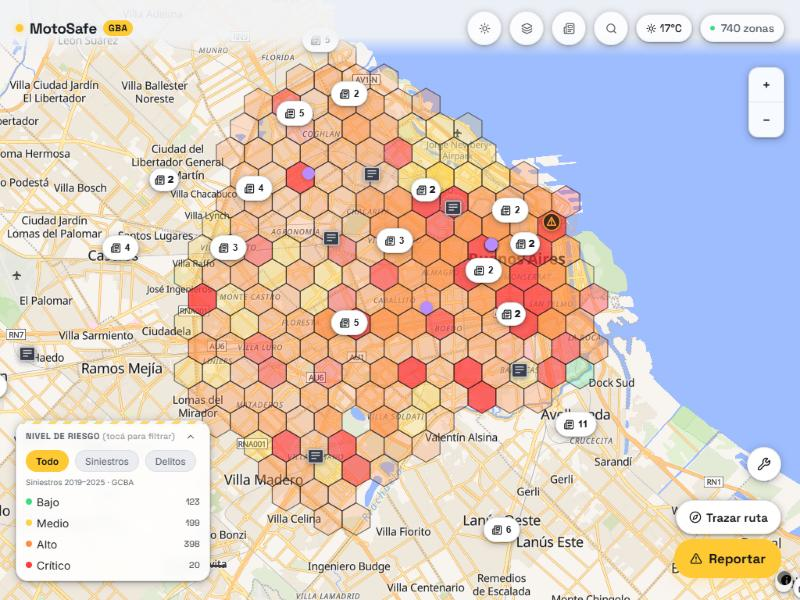
\includegraphics[width=0.9\textwidth,keepaspectratio]{figuras/image4.png}
    \caption{Vista del mapa con dos capas de riesgo activas simultáneamente (clusters de siniestros y de delitos). Captura de la aplicación real en producción.}
    \label{fig:4-4}
\end{figure}

\begin{figure}[H]
    \centering
    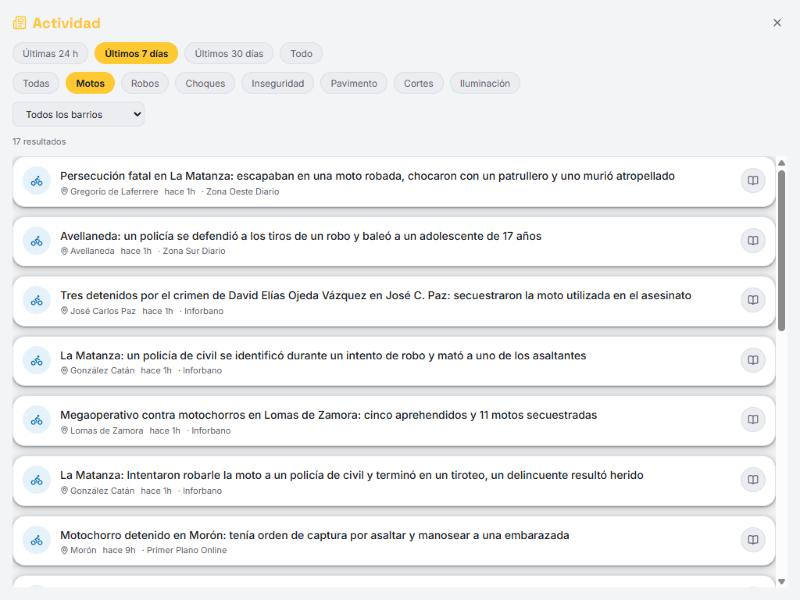
\includegraphics[width=0.9\textwidth,keepaspectratio]{figuras/image5.png}
    \caption{Panel de prensa con el filtro ``Motos'' aplicado, mostrando 17 resultados reales de los últimos 7 días. Captura de la aplicación real en producción.}
    \label{fig:4-5}
\end{figure}

\begin{figure}[H]
    \centering
    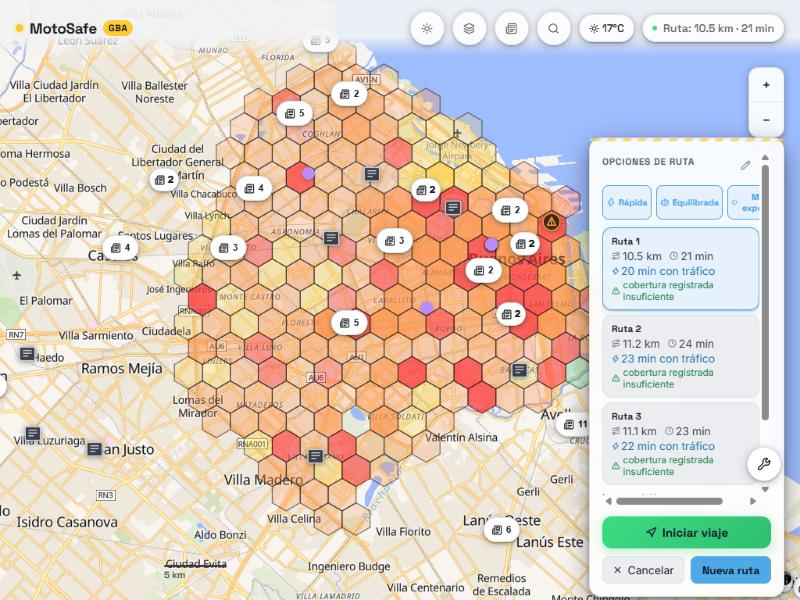
\includegraphics[width=0.9\textwidth,keepaspectratio]{figuras/image6.png}
    \caption{Comparador de tres rutas alternativas reales entre Monte Grande y Lomas de Zamora, con distancia, tiempo estimado y advertencia de cobertura registrada insuficiente por ruta. Captura de la aplicación real en producción.}
    \label{fig:4-6}
\end{figure}

\begin{figure}[H]
    \centering
    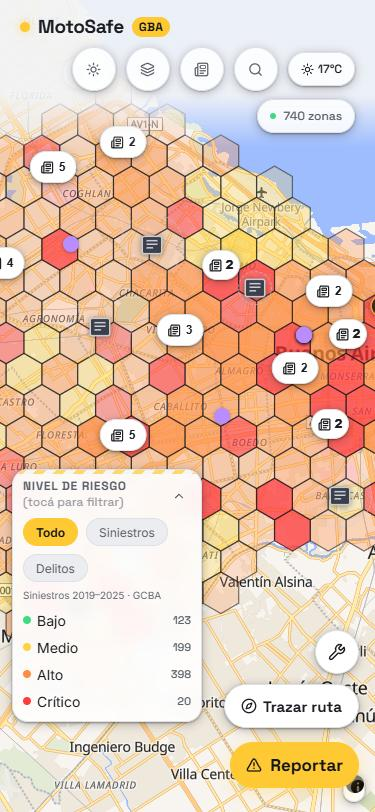
\includegraphics[height=0.65\textheight,keepaspectratio]{figuras/image7.png}
    \caption{Vista de la aplicación en un viewport móvil (375×812), con el mapa, la leyenda de nivel de riesgo y el botón de trazar ruta adaptados al ancho de pantalla. Captura de la aplicación real en producción.}
    \label{fig:4-7}
\end{figure}

Alcance mostrado en la demo (verificable en el código y en las capturas
incorporadas más arriba): mapa interactivo con capas de siniestros
históricos, hotspots viales, inseguridad general y prensa activables por
separado; comparador de hasta tres rutas con cobertura por fuente
mostrada como porcentaje o como "sin datos"; formulario de alta de
reporte comunitario con token de borrado entregado al autor del reporte.
Lo simulado o no implementado a esta fecha: aplicación móvil nativa y
cualquier notificación push o en tiempo real. El sistema de
autenticación de usuarios, simulado hasta la entrega anterior, ya está
implementado y corriendo en producción (detalle al final de 4.8).

\section{Estrategia de pruebas, control de versiones y despliegue}

Antes de que un cambio llegue al sistema en funcionamiento, el proyecto
pasa por varias capas de verificación automática pensadas para atajar
errores lo antes posible, en vez de depender de que alguien los note a
mano. La primera es el lint: un análisis del código que no lo ejecuta,
sino que lo revisa en busca de errores de sintaxis, variables sin usar o
patrones que suelen esconder bugs. Encima corre la suite de pruebas
automatizadas: funciones que ejercitan una parte puntual del sistema con
datos conocidos y comparan el resultado contra el esperado, de forma que
un cambio que rompa algo se detecta de inmediato y no cuando ya está en
producción. El frontend cuenta con 111 de estas pruebas (con Vitest)
sobre el cálculo de tiempo estimado, el riesgo geográfico, el riesgo de
ruta y el almacenamiento local del navegador; el backend cuenta con 168
(con pytest), que incluyen los casos de la cuota diaria de reportes, el
endpoint de métricas y los alias de localidad del extractor de prensa.

Un flujo de integración continua en GitHub Actions corre automáticamente
cada vez que se sube un cambio al repositorio: el frontend ejecuta lint,
la suite de pruebas con Vitest y el build de producción; el backend
instala las dependencias fijadas por hash (requirements.lock), levanta
un servicio PostgreSQL/PostGIS real y desechable para cada corrida, y
ejecuta la suite completa de pytest contra esa base, cubriendo así la
integración con la base de datos y no solo el código aislado. Un segundo
flujo, independiente del anterior, dispara el scraper de prensa cada
tres horas por cron en GitHub Actions (y también a demanda) contra la
base real de producción en Supabase.

El sistema corre en producción con migraciones SQL versionadas aplicadas
contra la base real de Supabase (las siete migraciones del esquema,
incluidas las del sistema de usuarios), con imágenes Docker de
producción en Render (mismo Dockerfile y mismo entrypoint.sh que en el
Compose local) y con los tres componentes accesibles públicamente
(motosafe-api.onrender.com, motosafe-web.onrender.com, y el scraper en
GitHub Actions). Quedan pendientes el dominio propio (hoy el HTTPS lo
resuelve el subdominio de Render) y un ciclo de backup y restauración
ensayado sobre la base real de Supabase; los límites de gasto activos no
aplican de la misma manera que en el plan original, porque toda la
operación corre en planes gratuitos sin cargo por uso que pueda exceder
un presupuesto.

\section{Limitaciones técnicas y evolución prevista}

Quedan pendientes las siguientes limitaciones técnicas. Los componentes
de interfaz de mayor tamaño todavía no separan del todo sus
responsabilidades internas. Falta ejecutar un ensayo de integridad de la
base de datos bajo un entorno de PostgreSQL aislado. Una limitación
señalada en una entrega anterior ya se cerró: la falta de fechas de
generación diferenciadas por capa, más allá de la prensa. El endpoint
/capas/cobertura expone hoy período y fecha de generación de cada capa
(siniestros, corredores, delitos general y por moto, además de prensa),
verificado visualmente en el navegador.

El extractor de prensa, aparte de las limitaciones abiertas, tiene
falsos positivos geográficos reproducibles (notas de fuera del área de
GBA geocodificadas con coordenadas del área de estudio) y todavía no se
midió su error geográfico en metros, porque esa medición requiere una
geocodificación externa independiente. Aun así, ya tiene una evaluación
real sobre datos reales, no solo una lista de pendientes: medido sobre
una corrida de 132 candidatas etiquetadas a mano contra su título (105
evaluables, 27 excluidas), dio una precisión temática de 0,84 y un
recall de 0,923.

La causa principal de la tasa de ubicación incompleta (localidades de
uso cotidiano en la prensa que todavía no estaban en el diccionario de
zonas del extractor) ya se corrigió agregando esas localidades como
alias del partido correspondiente, con pruebas de regresión nuevas que
evitan que vuelva a pasar inadvertida. La deduplicación semántica de
notas equivalentes entre medios distintos ya tiene una marca automática
funcionando (detalle en 4.6), pero falta confirmar su comportamiento
contra la base de producción real.

\section{Alternativas evaluadas y justificación}

Las alternativas tecnológicas descartadas se consolidan en la Tabla 4.5,
evaluadas contra los cinco criterios de 3.6 (representación geográfica
nativa, mantenibilidad por un solo desarrollador, persistencia y
consulta espacial eficiente, trazabilidad y cobertura de pruebas, y
costo sostenible). Los criterios de mantenibilidad y costo sostenible
son, en la práctica, los que más veces inclinan la balanza: aparecen en
casi todas las decisiones de esta tabla porque MotoSafe GBA se
desarrolla y va a operar con los recursos de una sola persona.

\begin{longtable}[]{@{}
  >{\raggedright\arraybackslash}p{(\columnwidth - 6\tabcolsep) * \real{0.2065}}
  >{\raggedright\arraybackslash}p{(\columnwidth - 6\tabcolsep) * \real{0.2609}}
  >{\raggedright\arraybackslash}p{(\columnwidth - 6\tabcolsep) * \real{0.2717}}
  >{\raggedright\arraybackslash}p{(\columnwidth - 6\tabcolsep) * \real{0.2609}}@{}}
\caption{Alternativas tecnológicas evaluadas y descartadas, por componente.}\label{tab:4-5}\\
\toprule\noalign{}
\begin{minipage}[b]{\linewidth}\raggedright
\textbf{Componente}
\end{minipage} & \begin{minipage}[b]{\linewidth}\raggedright
\textbf{Selección}
\end{minipage} & \begin{minipage}[b]{\linewidth}\raggedright
\textbf{Alternativa descartada}
\end{minipage} & \begin{minipage}[b]{\linewidth}\raggedright
\textbf{Motivo principal}
\end{minipage} \\
\midrule\noalign{}
\endfirsthead
\toprule\noalign{}
\begin{minipage}[b]{\linewidth}\raggedright
\textbf{Componente}
\end{minipage} & \begin{minipage}[b]{\linewidth}\raggedright
\textbf{Selección}
\end{minipage} & \begin{minipage}[b]{\linewidth}\raggedright
\textbf{Alternativa descartada}
\end{minipage} & \begin{minipage}[b]{\linewidth}\raggedright
\textbf{Motivo principal}
\end{minipage} \\
\midrule\noalign{}
\endhead
\bottomrule\noalign{}
\endlastfoot
Interfaz & React con Vite (aplicación de una sola página) & Aplicación
móvil nativa & No se necesita cámara, sensores ni otra función exclusiva
del dispositivo; una web evita distribuir por tienda \\
Mapa & MapLibre GL JS & Motores con mejor rendimiento sobre volúmenes
muy grandes de puntos & El volumen de datos del proyecto no lo
justifica; evita complejidad adicional pensada para otra escala \\
API y datos & FastAPI y PostgreSQL con PostGIS & Plataforma administrada
única (base de datos, backend y funciones) & Prioriza el control sobre
la lógica de servidor por sobre un menor trabajo de configuración
inicial \\
Modelo de gravedad & Random Forest (scikit-learn) & Red neuronal
profunda (por ejemplo, CNN) & Datos tabulares, no imágenes; no requiere
GPU ni el volumen de datos que una red profunda necesita para entrenar
bien \\
Mapas y ruteo externos & TomTom & Motor de ruteo propio & Mantener datos
viales actualizados excede el alcance de un proyecto de un solo
desarrollador \\
Arquitectura general & Monolito por capas con servicios externos
desacoplados & Microservicios & Equipo de una sola persona; el tráfico
actual no justifica coordinar despliegues independientes \\
Despliegue & Render (Web Services) + Supabase (PostgreSQL/PostGIS) +
GitHub Actions (cron del scraper) & Render (Blueprint declarativo, con
Postgres y cron propios) & La base de datos gratuita de Render vence a
los 30 días y su cron job es pago incluso en el plan más chico; Supabase
ofrece un plan gratuito sin vencimiento y GitHub Actions corre el cron
sin costo \\
\end{longtable}

La decisión de despliegue involucró en la práctica tres elecciones
distintas, revisadas con evidencia real antes de confirmarlas, no solo
en el papel. La primera es containerizar todo el sistema con Docker,
según se desarrolla en 3.8. La segunda es publicar la API y el sitio web
como Web Services de Render, descartando el Blueprint original (API,
Postgres y cron en un mismo despliegue) porque dos de sus tres piezas no
eran viables sin costo: la base de datos gratuita de Render vence a los
30 días, y su servicio de cron job es pago incluso en el plan más chico;
se migró la base a Supabase (gratuita, sin vencimiento, con PostGIS) y
el cron del scraper a GitHub Actions. La tercera, no prevista en el
diseño original, fue cambiar el envío de mail del sistema de usuarios de
SMTP a la API HTTP de Gmail, porque Render bloquea el tráfico saliente
por los puertos SMTP en su plan gratuito; se confirmó en vivo, probando
cada paso, que ninguna de las tres plataformas (Supabase, Render, Google
Cloud) pidió una tarjeta de crédito para esta configuración puntual. El
estado real y verificado de esta migración se reporta en 3.8 y 4.10.
